\section{Exact Restricted Decisions and Approximation Limits}\label{sec:allocation}
\subsection{A complete counterexample}
Consider $R(z_1,z_2,z_3)=1.2z_1+z_2+0.1z_3+3z_2z_3$. Exact isolated damage ranks $1>2>3$. With one protected bit,
\begin{equation}\label{eq:counterexample}
J_p(\{1\})=1.1p+3p^2,\quad J_p(\{2\})=1.3p,\quad J_p(\{3\})=2.2p.
\end{equation}
The optimal choice switches from bit 1 to bit 2 at $p=1/15$. There is no estimation error. This disproves universal isolated-ranking optimality, not the usefulness of static rankings on a particular network.
\begin{figure}[t]
\centering
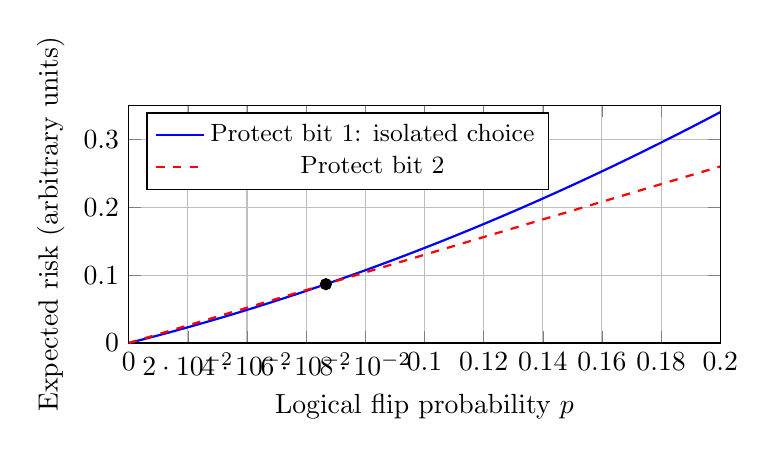
\begin{tikzpicture}
\begin{axis}[width=.75\linewidth,height=4.6cm,xlabel={Logical flip probability $p$},ylabel={Expected risk (arbitrary units)},xmin=0,xmax=.2,ymin=0,ymax=.35,grid=major,legend pos=north west,domain=0:.2,samples=101,legend style={font=\small}]
\addplot[thick,blue] {1.1*x+3*x^2};\addlegendentry{Protect bit 1: isolated choice}
\addplot[thick,red,dashed] {1.3*x};\addlegendentry{Protect bit 2}
\addplot[only marks,black] coordinates {(.0666666667,.0866666667)};
\end{axis}
\end{tikzpicture}
\caption{Analytical counterexample, not a measured neural-network result. The exact isolated ranking is optimal only below the crossing.}\label{fig:counterexample}
\Description{Two analytical risk curves cross at logical flip probability one fifteenth.}
\end{figure}

\subsection{Fixed global context and response-table reuse}
Let $P_0$ be a verified static mask, $C$ a frozen candidate pool of size $K$, and $r=|P_0\cap C|$. Fix $P_{\rm out}=P_0\setminus C$ and compare $P(Q)=P_{\rm out}\cup Q$ for every $Q\subseteq C$ with $|Q|=r$. The whole-network cardinality is unchanged. Draw $G$ only on coordinates outside $C\cup P_{\rm out}$ and evaluate $h_G(A)=R(G\cup A)$ for all $2^K$ candidate states. For $U=C\setminus Q$,
\begin{equation}\label{eq:exact-table}
J_G(Q)=\sum_{A\subseteq U}p^{|A|}(1-p)^{|U|-|A|}h_G(A),\qquad J_p(P(Q))=\E_G J_G(Q).
\end{equation}
One response table supports all eligible masks without further inference and retains every candidate interaction order. Exact candidate integration removes candidate-draw Monte Carlo noise, not outside-field or input-cohort uncertainty. The conditional equivalence between forcing a bit clean and suppressing it relies on the independent product law; it need not hold under correlated or fixed-count faults.

Masks are selected on model-selection cohorts and outside fields only. The original static mask, the exact-isolated comparator (largest signed clean single-bit effects on the selection cohort), and the minimum empirical integrated-risk mask are frozen before final evaluation. Exactness refers to executable effects and candidate integration; the selected mask minimizes a \emph{finite-field restricted} objective, not whole-network expected risk.

For a swap releasing $a\in P$ and protecting $b\notin P$, let $P'=(P\setminus\{a\})\cup\{b\}$. With the same Bernoulli background over coordinates unprotected under both masks,
\begin{equation}\label{eq:swap}
J_p(P')-J_p(P)=p\,\E_G[R(G\cup\{a\})-R(G\cup\{b\})].
\end{equation}
Final comparisons use this paired-swap identity along fixed paths; all path steps are summed within a master field before uncertainty is calculated. It remains valid for scalar cohort AUC. It does not assume an additive per-input risk or implement a new optimizer.

\subsection{An exact attribution of decision differences}\label{sec:decomposition}
On the \emph{same} selection cohort define $R_0=R(\varnothing)$, $d_b^0=R(\{b\})-R_0$, and $d_b^G=h_G(\{b\})-h_G(\varnothing)$. Then
\begin{align}\label{eq:decomposition}
J_G(Q)={}&\underbrace{R_0+p\sum_{b\in U}d_b^0}_{\text{clean isolated prediction}}
+\underbrace{h_G(\varnothing)-R_0}_{\text{background intercept}}\nonumber\\
&+\underbrace{p\sum_{b\in U}(d_b^G-d_b^0)}_{\text{outside-background correction}}
+\underbrace{J_G(Q)-h_G(\varnothing)-p\sum_{b\in U}d_b^G}_{\text{within-candidate correction}}.
\end{align}
The intercept cancels between masks. The remaining signed terms close exactly for every equal-budget contrast. Averaging absolute terms and signed terms answers different questions; cancellation can hide heterogeneous field effects. This is algebraic attribution, not proof that neural redundancy or gating caused an architectural difference.

Importantly, $d_b^G$ forces \emph{all other candidates clean}. Its outside-field mean is not the full $V_b$ in Eq.~\eqref{eq:prob-gradient}, which also averages unprotected candidate faults. For $h(A)=\mathbf1\{\{1,2,3\}\subseteq A\}$, every singleton response is zero but the full conditional vulnerability is $p^2$. A $K+1$-state approximation cannot be renamed an exact conditional oracle.

\subsection{Bounded-risk error and restricted regret}\label{sec:bounds}
Write $A_p(Q)=\E h_G(\varnothing)+p\sum_{b\in U}\E d_b^G$, and $E_{\ge2}(Q)=J_p(P(Q))-A_p(Q)$. If $0\le R\le L$ and $m=K-r\ge2$, then
\begin{equation}\label{eq:bound}
|E_{\ge2}(Q)|\le\epsilon_m=Lmp[1-(1-p)^{m-1}].
\end{equation}
The remainder is zero for $m\le1$. The bound is sharp without monotonicity assumptions: $h(\varnothing)=L$, singleton risks zero, and all multi-fault risks $L$ attain it. In particular, replacing the right side by $L\Prob(|A|\ge2)$ is invalid; the singleton linearization can overshoot the risk range. The proof is in Appendix~\ref{app:math}.

If $Q_A$ minimizes the outside-additive function and $Q_*$ minimizes exact expected risk in the same restricted family, the regret is at most $\min(L,2\epsilon_m)$. For $n$ independent outside fields, define $t=L\sqrt{2\log(2K/\alpha)/n}$. Hoeffding's inequality and an equal-budget cancellation argument give, with probability at least $1-\alpha$,
\begin{equation}\label{eq:samplebound}
J_p(P(\widehat Q_A))-J_p(P(Q_*))
\le \min\{L,2\epsilon_m+2p\min(r,K-r)t\}.
\end{equation}
This conditions on a frozen pool, model and cohort. Shared fields across bits are allowed; independent fields across observations are required. The approximation bias and field-estimation uncertainty are separate.

A globally certified bound $\kappa_{bc}$ on every contextual second difference yields the alternative $p^2\sum_{b<c\in U}\kappa_{bc}$. Maxima over recorded fields certify only those recorded fields. Empty-context pair differences alone cannot bound pure third-order effects. The inequalities clarify limits, but a numerically loose certificate is not evidence that a small observed decision difference is practically resolved.
